%%%%%%%%%%%%%%%%%%%%%%%%%%%%%%%%%%%%%%
%% Frame
%%%%%%%%%%%%%%%%%%%%%%%%%%%%%%%%%%%%%%

\begin{frame}[t]
	\frametitle{Introduction}
	\framesubtitle{~~}  %% needed for proper positioning of the logo ...

\begin{figure}[h]
	\centering
	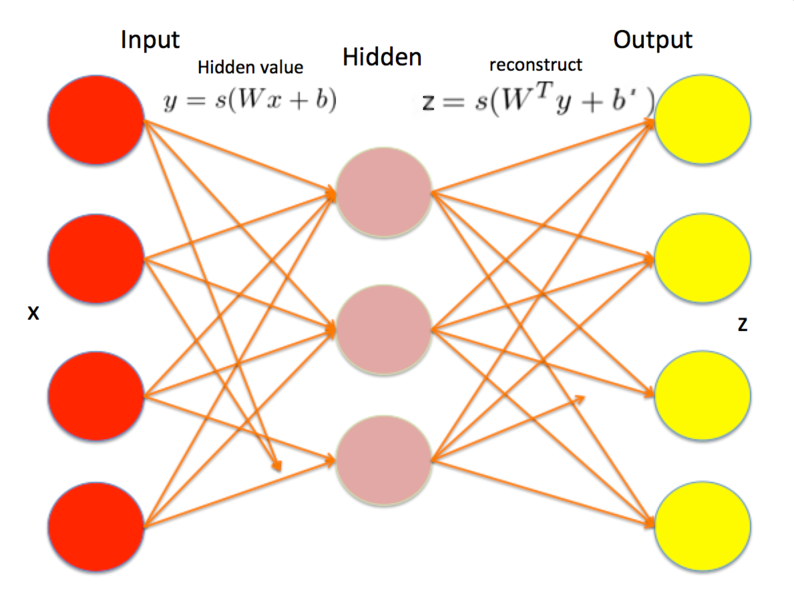
\includegraphics[width=0.7\linewidth]{autoencoder.png}
	\caption{Overview of an autoencoder and its encoding, decoding stages. The weight matrix of the decoding stage is the transpose of the weight matrix of the encoding stage.}
	\label{fig:autoencoder}
\end{figure}


\end{frame}

%%%%%%%%%%%%%%%%%%%%%%%%%%%%%%%%%%%%%%
%% Frame
%%%%%%%%%%%%%%%%%%%%%%%%%%%%%%%%%%%%%%

\begin{frame}[t]
	\frametitle{Introduction}
	\framesubtitle{~~}  %% needed for proper positioning of the logo ...
	\begin{itemize}
		\item Traditional autoencoders
		\item Denoising autoencoders
		\item Stochastic Gradient Descent (SGD) and backpropogation
		\item Genetic algorithms
	\end{itemize}


\end{frame}

